\subsection{Least Common Multiple of Polynomials} 
To find the LCD for rational expressions, we must be able to find the least common multiple (LCM) of two (or more) polynomials.
\begin{procedure}{Finding Least Common Multiple for Polynomials}
\begin{enumerate*}
\item Factor all denominators.
\item Build the LCM:
\begin{itemize*}
\item Must have all factors that appear in any denominator.
\item If factors appear with different powers, take the highest power.
\end{itemize*}
\end{enumerate*}
\end{procedure}
\begin{Note} The LCM and the GCF (greatest common factor) are found in similar ways, but the GCF must be a factor of each polynomial, and each polynomial must be a factor of the LCM.
\begin{center}
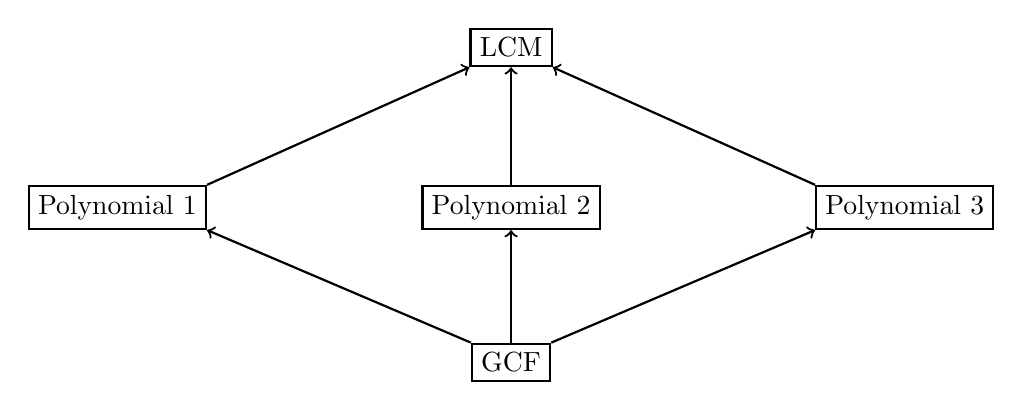
\begin{tikzpicture}[every node/.style={rectangle,draw,thick,anchor=base}]
\node (lcd) at (0,2) {LCM};
\node (gcf) at (0,-2) {GCF};
\foreach \x in {1,2,3} {
	\node (poly-\x) at (\x*5-10,0) {Polynomial \x};
}
\draw[->,thick] (gcf.north west) -- (poly-1.south east);
\draw[->,thick] (gcf.north) -- (poly-2.south);
\draw[->,thick] (gcf.north east) -- (poly-3.south west);
\draw[->,thick] (poly-1.north east) -- (lcd.south west);
\draw[->,thick] (poly-2.north) -- (lcd.south);
\draw[->,thick] (poly-3.north west) -- (lcd.south east);
\end{tikzpicture}
\end{center}
\end{Note}
%\begin{Note}We'll say LCM when we're just thinking about the polynomials, LCD when we're thinking of them as denominators. They're the same thing, just in different contexts.\end{Note}
\begin{Example}
Find the least common multiple of $3x^2y$, $2x^5z$, and $9xy^3$.
\begin{lpic}{}{2}
\regtextleft{0.25}{-2}{$\mathrm{LCM}={}$};
\end{lpic}
\end{Example}
\begin{Example}
Find the least common multiple of the three polynomials below. Leave the answer in factored form.
\begin{lpic}{}{10}
\foreach \y/\exp in {1/6x^2-9x-6,4/3x^4-12x^3+12x^2,7/2x^4+x^3-8x^2-4x,10/\mathrm{LCM}} {
	\regtextleft{0.25}{-\y}{$\exp={}$};
}
\end{lpic}
\end{Example}